\PassOptionsToPackage{unicode=true}{hyperref} % options for packages loaded elsewhere
\PassOptionsToPackage{hyphens}{url}
\documentclass[11pt,ignorenonframetext,aspectratio=169]{beamer}
\IfFileExists{pgfpages.sty}{\usepackage{pgfpages}}{}
\setbeamertemplate{caption}[numbered]
\setbeamertemplate{caption label separator}{: }
\setbeamercolor{caption name}{fg=normal text.fg}
\beamertemplatenavigationsymbolsempty
\usepackage{lmodern}
\usepackage{amssymb,amsmath}
\usepackage{ifxetex,ifluatex}
\usepackage{fixltx2e} % provides \textsubscript
\ifnum 0\ifxetex 1\fi\ifluatex 1\fi=0 % if pdftex
  \usepackage[T1]{fontenc}
  \usepackage[utf8]{inputenc}
\else % if luatex or xelatex
  \ifxetex
    \usepackage{mathspec}
  \else
    \usepackage{fontspec}
\fi
\defaultfontfeatures{Ligatures=TeX,Scale=MatchLowercase}







\fi

  \usetheme[sectionpage=progressbar, titleformat=regular,
numbering=counter, block=fill]{metropolis}






% use upquote if available, for straight quotes in verbatim environments
\IfFileExists{upquote.sty}{\usepackage{upquote}}{}
% use microtype if available
\IfFileExists{microtype.sty}{%
  \usepackage{microtype}
  \UseMicrotypeSet[protrusion]{basicmath} % disable protrusion for tt fonts
}{}


\newif\ifbibliography
  \usepackage[round]{natbib}
  \bibliographystyle{plainnat}


\hypersetup{
      pdftitle={Heterosis and inbreeding depression},
        pdfauthor={Deependra Dhakal},
          pdfborder={0 0 0},
    breaklinks=true}
%\urlstyle{same}  % Use monospace font for urls







% Prevent slide breaks in the middle of a paragraph:
\widowpenalties 1 10000
\raggedbottom

  \AtBeginPart{
    \let\insertpartnumber\relax
    \let\partname\relax
    \frame{\partpage}
  }
  \AtBeginSection{
    \ifbibliography
    \else
      \let\insertsectionnumber\relax
      \let\sectionname\relax
      \frame{\sectionpage}
    \fi
  }
  \AtBeginSubsection{
    \let\insertsubsectionnumber\relax
    \let\subsectionname\relax
    \frame{\subsectionpage}
  }



\setlength{\parindent}{0pt}
\setlength{\parskip}{6pt plus 2pt minus 1pt}
\setlength{\emergencystretch}{3em}  % prevent overfull lines
\providecommand{\tightlist}{%
  \setlength{\itemsep}{0pt}\setlength{\parskip}{0pt}}

  \setcounter{secnumdepth}{0}


  \usepackage{setspace}
  \usepackage{wasysym}
  % \usepackage{fontenc}
  \usepackage{booktabs,siunitx}
  \usepackage{longtable}
  \usepackage{array}
  \usepackage{multirow}
  \usepackage{wrapfig}
  \usepackage{float}
  \usepackage{colortbl}
  \usepackage{pdflscape}
  \usepackage{tabu}
  \usepackage{threeparttable}
  \usepackage{threeparttablex}
  \usepackage[normalem]{ulem}
  \usepackage{makecell}
  \usepackage{xcolor}
  \usepackage{tikz} % required for image opacity change
  \usepackage[absolute,overlay]{textpos} % for text formatting
  \usepackage[skip=0.333\baselineskip]{caption}
  % \usepackage{newtxtext,newtxmath}% better than txfonts   
  \usepackage[english]{babel}
  \usepackage{pgfpages}

  \sisetup{per-mode=symbol}

  % % Added by CII
  % \usepackage[format=hang,labelfont=bf,margin=0.5cm,justification=centering]{caption}
  % \captionsetup{font=small,width=0.9\linewidth,labelfont=small,textfont={small}}
  % % End of CII addition

  % \usepackage{subcaption}
  % \newcommand{\subfloat}[2][need a sub-caption]{\subcaptionbox{#1}{#2}}

  \captionsetup[sub]{font=footnotesize,labelfont=footnotesize,textfont=footnotesize}
  % \captionsetup[subfigure]{font=small,labelfont=small,textfont=small}
  % \captionsetup[subfloat]{font=scriptsize,labelfont=scriptsize,textfont=scriptsize}

  % this font option is amenable for beamer, although these are global settings
  \setbeamerfont{caption}{size=\tiny}
  % \setbeamerfont{subcaption}{size=\tiny} % this does not chage subfloat fonts
  % \setbeamerfont{subfloat}{size=\tiny} % this does not change subfloat fonts
   
   % use single line spacing ?
  \singlespacing

  % use cslreferences environment
  % this is revised as of Oct, 2022 (https://stackoverflow.com/questions/59193797/pandocs-environment-cslreferences-undefined-when-knitting-rmarkdown-to-pdf-in-r)
  \newlength{\cslhangindent}
  \setlength{\cslhangindent}{1.5em}
  \newenvironment{CSLReferences}%
    {\setlength{\parindent}{0pt}%
    \everypar{\setlength{\hangindent}{\cslhangindent}}\ignorespaces}%
    {\par}


  \newcommand{\bcolumns}{\begin{columns}[T, onlytextwidth]}
  \newcommand{\ecolumns}{\end{columns}}

  \newcommand{\bdescription}{\begin{description}}
  \newcommand{\edescription}{\end{description}}

  \newcommand{\bitemize}{\begin{itemize}}
  \newcommand{\eitemize}{\end{itemize}}

  \title[]{Heterosis and inbreeding depression}


  \author[
        Deependra Dhakal
    ]{Deependra Dhakal}

  \institute[
    ]{
    Agriculture and Forestry University\\
\textit{ddhakal.rookie@gmail.com}\\
\url{https://rookie.rbind.io}
    }

\date[
      
  ]{
    }


\begin{document}

% Hide progress bar and footline on titlepage
  \begin{frame}[plain]
  \titlepage
  \end{frame}



\hypertarget{hybrid-vigour-heterosis}{%
\section{Hybrid vigour (Heterosis)}\label{hybrid-vigour-heterosis}}

\begin{frame}{}
\protect\hypertarget{section}{}
\begin{itemize}
\tightlist
\item
  Hybrid vigor may be defined as the increase in size, vigor, fertility,
  and overall productivity of a hybrid plant over the mid-parent value
  (average performance of the two parents).
\item
  It is calculated as the difference between the crossbred and inbred
  means:
\end{itemize}

\[\text{Hybrid vigour} = \frac{F_1-\frac{(P_1+P_2)}{2}}{\frac{(P_1+P_2)}{2}}\]

\begin{itemize}
\tightlist
\item
  The estimate is usually calculated as a percentage.
\item
  The synonymous term, heterosis, was coined by G.H. Shull.
\item
  Advantageous hybrid vigor is observed more frequently when breeders
  cross parents that are genetically diverse; When two inbred lines of
  outbred species are crossed.
\item
  The practical definition of heterosis is hybrid vigor that greatly
  exceeds the better or higher parent in a cross.
\item
  Hybrid breeding in maize quadrupled yields of maize in US between
  1930s and 1970s.
\end{itemize}
\end{frame}

\hypertarget{inbreeding-depression}{%
\section{Inbreeding depression}\label{inbreeding-depression}}

\begin{frame}{}
\protect\hypertarget{section-1}{}
\begin{itemize}
\tightlist
\item
  Inbreeding depression is reduction in fitness as a direct result of
  inbreeding.
\item
  In theory, the heterosis observed on crossing is expected to be equal
  to the depression upon inbreeding, considering a large number of
  crosses between lines derived from a single base population.
\item
  In practice, plant breeders are interested in heterosis expressed by
  specific crosses between selected parents, or between populations that
  have no known common origin.
\item
  Reduction in fitness is usually manifested as a reduction in vigor,
  fertility, and productivity.
\item
  The effect is more severe in the early generations (5-8).
\item
  Plants including onions, sunflower, cucurbits, and rye are more
  tolerant of inbreeding with minimal consequences of inbreeding
  depression.
\item
  Plants such as alfalfa and carrot are highly intolerant of inbreeding.
\end{itemize}
\end{frame}

\begin{frame}{}
\protect\hypertarget{section-2}{}
\begin{itemize}
\tightlist
\item
  Inbreeding is measured by the coefficient of inbreeding (F), which is
  the probability of identity of alleles by descent. The range of F is
  zero (no inbreeding; random mating) to one (prolonged selfing).
\item
  An unfit (deleterious) recessive allele is fairly quickly reduced in
  frequency but declines slowly thereafter.
\item
  On the other hand, an unfit dominant allele is rapidly eliminated from
  the population, while an intermediate allele is reduced more rapidly
  than a recessive allele because the former is open to selection in the
  heterozygote.
\item
  The consequence of these outcomes is that unfit dominant or
  intermediate alleles are rare in cross-breeding populations, while
  unfit recessive alleles persist because they are protected by their
  recessiveness.
\end{itemize}
\end{frame}

\begin{frame}{}
\protect\hypertarget{section-3}{}
\begin{itemize}
\tightlist
\item
  In Figure \ref{fig:inbreeding-coefficient} (a) there is no inbreeding
  because there is no common ancestral pathway to the individual, A
  (i.e., all parents are different).
\item
  However, in Figure \ref{fig:inbreeding-coefficient} (b) inbreeding
  exists because B and C have common parents (D and E), that is, they
  are full sibs.
\item
  To calculate the amount of inbreeding, the standard pedigree is
  converted to an arrow diagram, as shown in Figure
  \ref{fig:inbreeding-coefficient} (c).
\item
  Each individual contributes 1/2 of its genotype to its offspring. The
  \emph{coefficient of relationship} (R) is calculated by summing up all
  the pathways between two individuals through a common ancestor as:
  \(R_{BC} = \sum{\left(\frac{1}{2}\right)^s}\) , where s is the number
  of steps (arrows) from B to the common ancestor and back to C. For
  example, B and C probably inherited \((1/2)(1/2) = 1/4\) of their
  genes in common through ancestor D. Similarly, B and C probably
  inherited 1/4 of their genes in common through ancestor E.
\item
  The coefficient of relationship between B and C, as a result of common
  ancestry, is hence \(R_{BC} = 1/4 + 1/4 = 1/2 = 50\%\)
\end{itemize}
\end{frame}

\begin{frame}{}
\protect\hypertarget{section-4}{}
\begin{figure}

{\centering 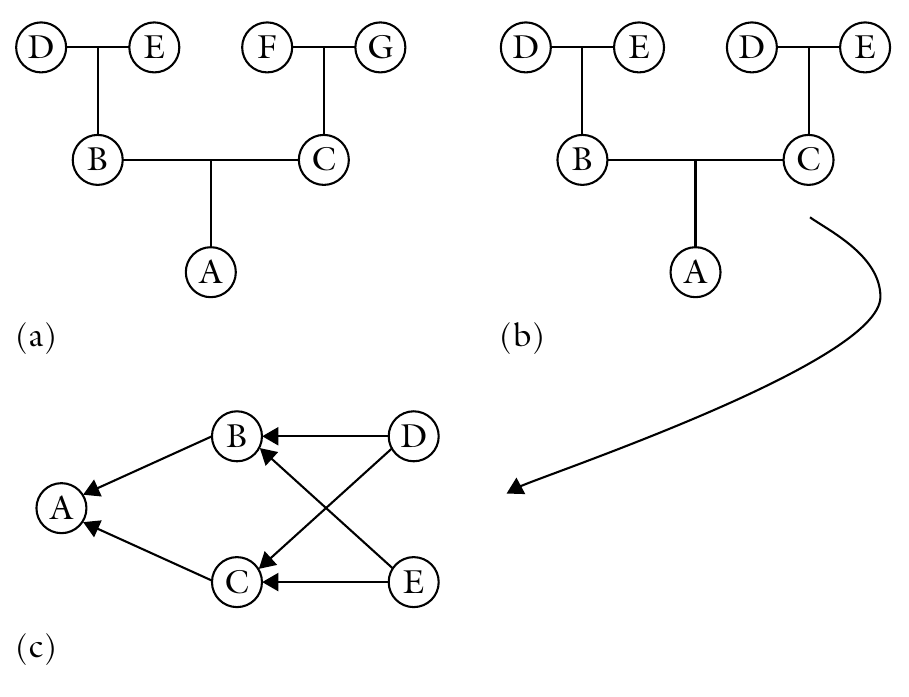
\includegraphics[width=0.6\linewidth]{./images/arrow_diagram} 

}

\caption{Pedigree diagrams can be drawn in the standard form (a, b) or converted to into an arrow diagram (c).}\label{fig:inbreeding-coefficient}
\end{figure}
\end{frame}

\hypertarget{genetic-basis-of-heterosis}{%
\section{Genetic basis of heterosis}\label{genetic-basis-of-heterosis}}

\begin{frame}{}
\protect\hypertarget{section-5}{}
\begin{itemize}
\tightlist
\item
  To explain the genetic basis for why fitness lost on inbreeding tends
  to be restored upon crossing, two theories have been proposed.

  \begin{itemize}
  \tightlist
  \item
    Dominance theory: C.G. Davenport in 1908 and later by I.M. Lerner,
  \item
    Overdominance theory: Shull in 1908 and later by K. Mather and J.L.
    Jinks.
  \end{itemize}
\item
  A third theory, the mechanism of epistasis (non-allelic gene
  interactions), has also been proposed.
\end{itemize}
\end{frame}

\begin{frame}{Dominance theory}
\protect\hypertarget{dominance-theory}{}
\small

\begin{itemize}
\tightlist
\item
  Assumes that vigor in plants is conditioned by dominant alleles,
  recessive alleles being deleterious or neutral in effect.
\item
  \alert{A genotype with more dominant alleles will be more vigorous than one with few dominant alleles.}
\item
  Consequently, crossing two parents with complementary dominant alleles
  will concentrate more favorable alleles in the hybrid than either
  parent.
\item
  Inbreeding depression occurs upon selfing because the deleterious
  recessive alleles that were protected in the heterozygous condition
  (\alert{heterozygous advantage}) become homozygous and are expressed.
\item
  Assume that each dominant genotype contributes 2 units to the
  phenotype, while a recessive genotype contributes 1 unit. A cross
  between two inbred parents would result in:
\end{itemize}

\begin{center}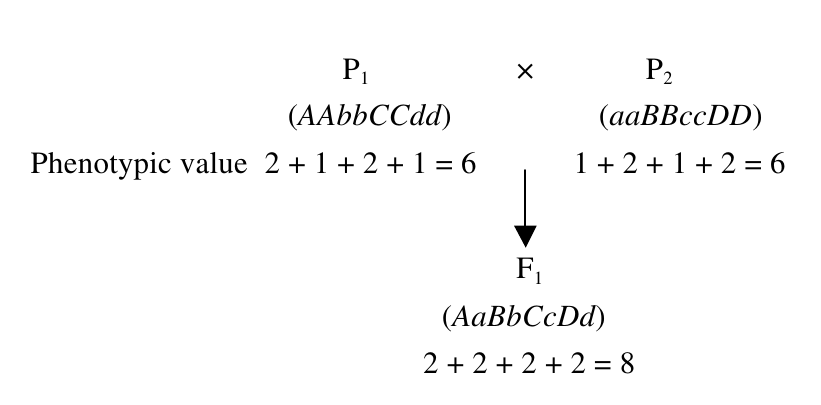
\includegraphics[width=0.4\linewidth]{./images/dominance_theory} \end{center}
\end{frame}

\begin{frame}{Overdominance theory}
\protect\hypertarget{overdominance-theory}{}
\small

\begin{itemize}
\tightlist
\item
  The phenomenon of the heterozygote being superior to the homozygote
  (i.e., heterozygosity \emph{per se} is assumed to be responsible for
  heterosis).
\item
  Theory assumes that the alleles of a gene (e.g., A, a) are contrasting
  but each has a different favorable effect in the plant.
\item
  A genotype with more heterozygous loci would be more vigorous than one
  with less heterozygotes.
\item
  Consider a quantitative trait conditioned by four loci, and assume
  that recessive, heterozygote, and homozygote dominants contribute 1,
  2, and 1.5 units to the phenotypic value, respectively:
\end{itemize}

\begin{center}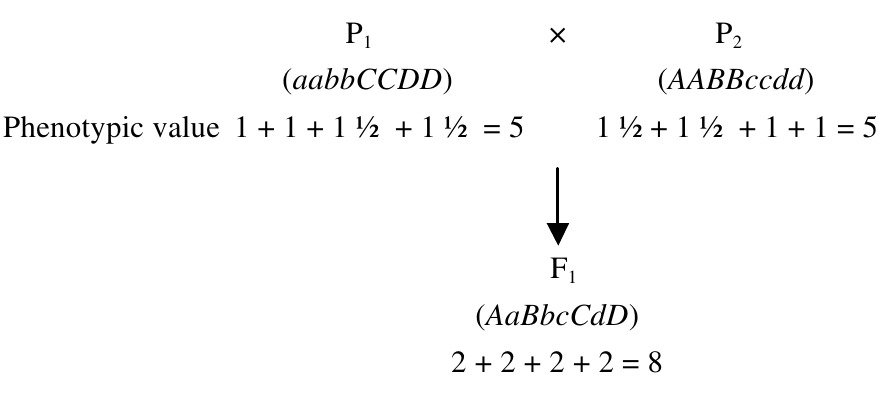
\includegraphics[width=0.5\linewidth]{./images/overdominance_theory} \end{center}
\end{frame}

\hypertarget{biometrics-of-heterosis}{%
\section{Biometrics of heterosis}\label{biometrics-of-heterosis}}

\begin{frame}{Biometrics of heterosis}
\begin{block}{Better parent heterosis (Heterobeltiosis)}
\protect\hypertarget{better-parent-heterosis-heterobeltiosis}{}
\[\large \text{Hybrid vigour} = \frac{F_1-\text{Better parent}}{\text{Better parent}}\]
\end{block}

\begin{block}{Mid parent heterosis}
\protect\hypertarget{mid-parent-heterosis}{}
\[\large \text{Hybrid vigour} = \frac{F_1-\frac{(P_1+P_2)}{2}}{\frac{(P_1+P_2)}{2}}\]
\end{block}

\begin{block}{Commercial heterosis}
\protect\hypertarget{commercial-heterosis}{}
\[\large \text{Hybrid vigour} = \frac{F_1-\text{Commercial hybrid}}{\text{Commercial hybrid}}\]
\end{block}
\end{frame}

\hypertarget{types-of-hybrids}{%
\section{Types of hybrids}\label{types-of-hybrids}}

\begin{frame}{}
\protect\hypertarget{section-6}{}
\begin{itemize}
\tightlist
\item
  Commercial applications of hybrid breeding started with a cross of two
  inbred lines (a single cross - AxB) and later shifted to the more
  economic double cross, ({[}AxB{]}x{[}CxD{]}) and then back to a single
  cross.
\item
  Other parent combinations in hybrid development have been proposed,
  including the three-way cross ({[}AxB{]}xC) and modified versions of
  the single cross, in which closely related crosses showed that the
  single cross was superior in performance to the other two in terms of
  average yield.
\item
  However, it was noted also that the genotype x environment interaction
  (hybrid x environment) variability was more than twice that for the
  double crosses, while the mean variability for the three-way cross
  being intermediate.
\end{itemize}
\end{frame}

\begin{frame}{}
\protect\hypertarget{section-7}{}
\begin{itemize}
\tightlist
\item
  This indicated that the single crosses were more sensitive or
  responsive to environmental conditions than the other crosses.
\item
  Whereas high average yield is important to the producer, consistency
  in performance across years and locations (i.e., yield stability) is
  also important.
\item
  Double and three-way crosses have a more genetically divergent
  population for achieving buffering.
\item
  Today commercial hybrids are predominantly single cross, of best
  combining parental inbred lines.
\item
  For outline of mating scheme, See Lecture 7 on ``Hybridization
  techniques and its consequences''.
\end{itemize}
\end{frame}

\begin{frame}{Breeding of CMS hybrids}
\protect\hypertarget{breeding-of-cms-hybrids}{}
\bcolumns
\column{0.35\textwidth}
\begin{figure}

{\centering 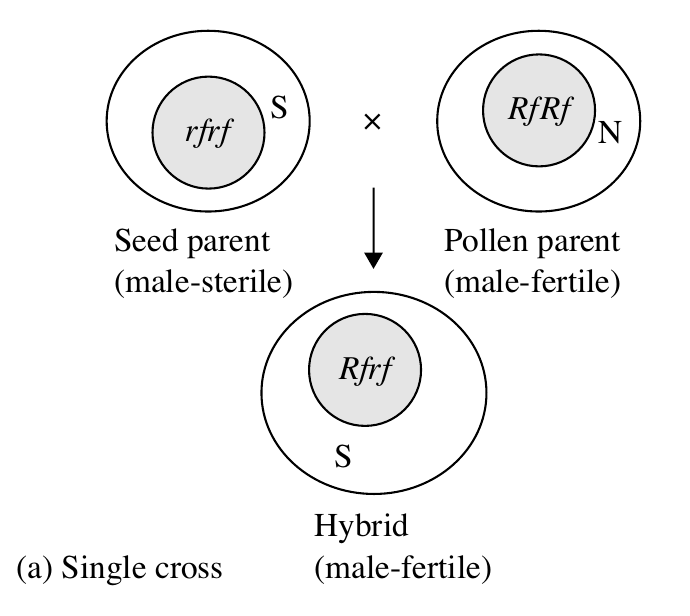
\includegraphics[width=0.9\linewidth]{./images/cms_hybrids_single} 

}

\caption{Breeding of single cross hybrid using CMS system. N, normal cytoplasm; S, sterile cytoplasm. Parent A=A-line; parent B=B-line, and parent D=R-line.}\label{fig:cms-hybrids-single}
\end{figure}

\column{0.65\textwidth}
\begin{figure}

{\centering 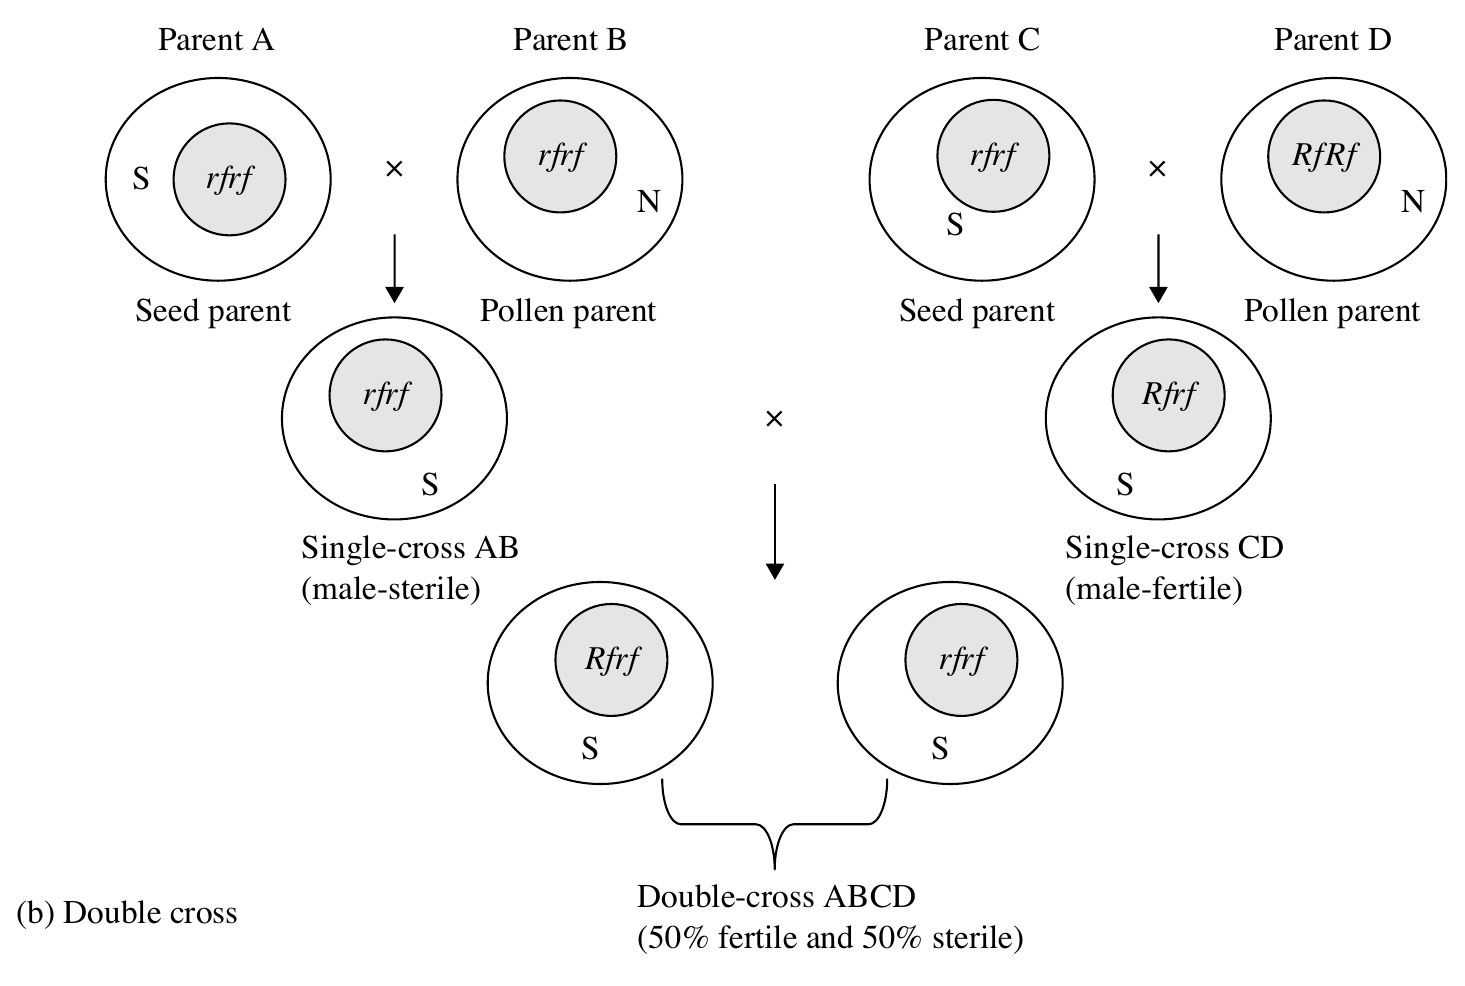
\includegraphics[width=0.98\linewidth]{./images/cms_hybrids_double} 

}

\caption{Breeding of double cross hybrid using CMS system.}\label{fig:cms-hybrids-double}
\end{figure}

\ecolumns
\end{frame}

\hypertarget{bibliography}{%
\section{Bibliography}\label{bibliography}}

\begin{frame}{}
\protect\hypertarget{section-8}{}
\end{frame}

          \begin{frame}[allowframebreaks]{}
    \bibliographytrue
    \bibliography{../bibliographies.bib}
    \end{frame}
  


\end{document}
